% standalone source of the reader-architecture figure (pdflatex architecture.tex); included as figures/architecture.pdf.
\documentclass[border=3pt]{standalone}
\usepackage{amsmath,amssymb}
\usepackage{tikz}
\usetikzlibrary{positioning,arrows.meta,fit,calc,backgrounds}
\begin{document}
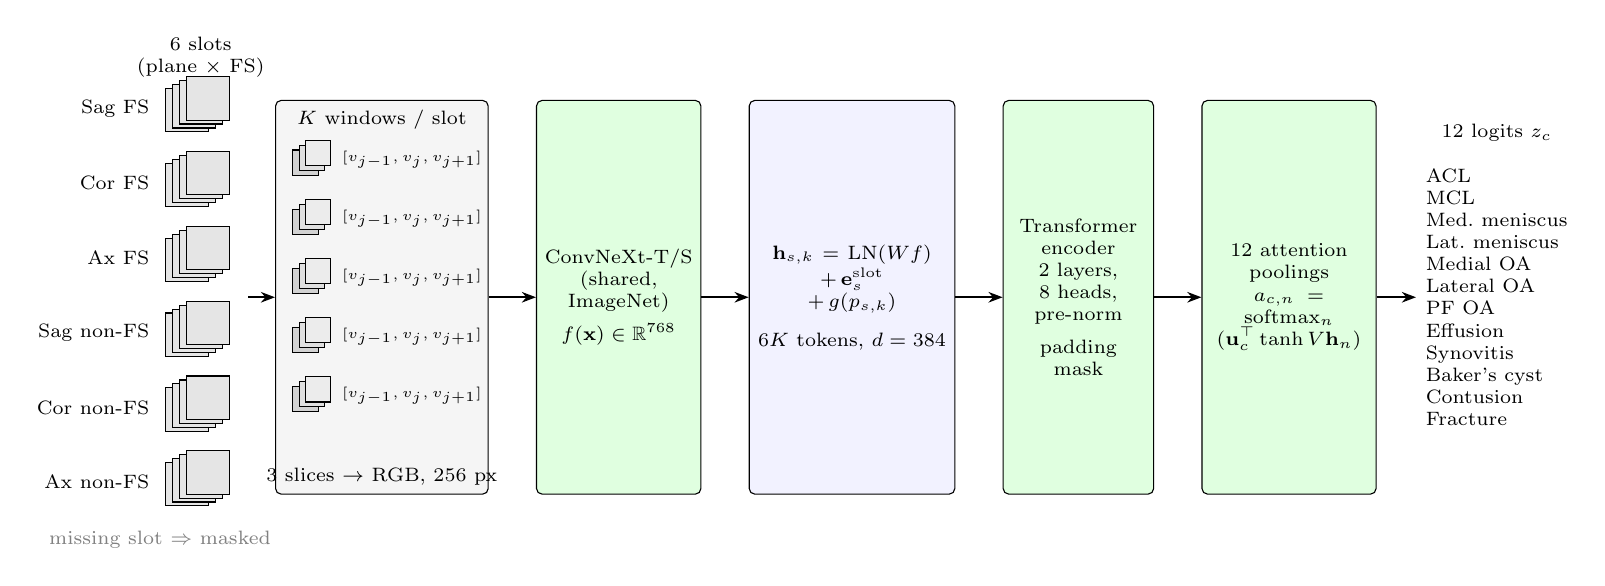
\begin{tikzpicture}[
  font=\scriptsize,
  arr/.style={-{Stealth[length=1.8mm]}, semithick},
  blk/.style={draw, rounded corners=2pt, align=center, minimum height=8mm, inner sep=3pt, fill=white},
  enc/.style={blk, fill=green!12, minimum width=17mm},
  head/.style={blk, fill=green!12},
  tok/.style={draw, fill=blue!15, minimum width=2.2mm, minimum height=5mm, inner sep=0pt},
  slice/.style={draw, fill=gray!20}]

% ---- six slots: each drawn as a small stack of slices -------------------------------------------
\foreach \i/\name in {0/{Sag FS}, 1/{Cor FS}, 2/{Ax FS}, 3/{Sag non-FS}, 4/{Cor non-FS}, 5/{Ax non-FS}} {
  \begin{scope}[shift={(0,-\i*0.95)}]
    \foreach \k in {0,1,2,3} {
      \draw[slice] ({0.09*\k},{0.05*\k}) rectangle ++(0.55,0.55);
    }
    \node[anchor=east, align=right] at (-0.08,0.3) {\name};
  \end{scope}
}
\node[align=center] at (0.45,0.95) {6 slots\\(plane $\times$ FS)};
\node[align=left, gray, anchor=north west] at (-1.6,-4.95) {missing slot $\Rightarrow$ masked};

% ---- windows ------------------------------------------------------------------------------------
\node[blk, minimum width=27mm, minimum height=50mm, fill=gray!8] (win) at (2.75,-2.1) {};
\node[anchor=north] at (win.north) {$K$ windows / slot};
\foreach \j in {0,...,4} {
  \begin{scope}[shift={(1.62,{-0.55-\j*0.75})}]
    \draw[fill=gray!35] (0,0) rectangle (0.32,0.32);
    \draw[fill=gray!25] (0.08,0.06) rectangle (0.40,0.38);
    \draw[fill=gray!15] (0.16,0.12) rectangle (0.48,0.44);
    \node[anchor=west, font=\tiny] at (0.5,0.2) {$[v_{j-1},v_j,v_{j+1}]$};
  \end{scope}
}
\node[anchor=south, align=center] at (win.south) {3 slices $\to$ RGB, 256 px};
\draw[arr] (1.05,-2.1) -- (win.west);

% ---- encoder ------------------------------------------------------------------------------------
\node[enc, right=6mm of win, minimum height=50mm] (cnx) {ConvNeXt-T/S\\(shared,\\ImageNet)\\[4pt]$f(\mathbf{x})\in\mathbb{R}^{768}$};
\draw[arr] (win.east) -- (cnx.west);

% ---- token construction -------------------------------------------------------------------------
\node[blk, right=6mm of cnx, minimum height=50mm, text width=24mm, fill=blue!5] (emb) {$\mathbf{h}_{s,k}=\mathrm{LN}(Wf)$\\$+\,\mathbf{e}^{\mathrm{slot}}_s$\\$+\,g(p_{s,k})$\\[6pt]$6K$ tokens, $d=384$};
\draw[arr] (cnx.east) -- (emb.west);

% ---- transformer --------------------------------------------------------------------------------
\node[head, right=6mm of emb, minimum height=50mm, text width=17mm] (tf) {Transformer\\encoder\\2 layers,\\8 heads,\\pre-norm\\[4pt]padding\\mask};
\draw[arr] (emb.east) -- (tf.west);

% ---- per-finding attention pooling --------------------------------------------------------------
\node[head, right=6mm of tf, minimum height=50mm, text width=20mm] (pool) {12 attention\\poolings\\$a_{c,n}=\operatorname{softmax}_n$\\$(\mathbf{u}_c^{\top}\tanh V\mathbf{h}_n)$};
\draw[arr] (tf.east) -- (pool.west);

% ---- outputs ------------------------------------------------------------------------------------
\node[right=5mm of pool, align=left, anchor=west] (out) {ACL\\MCL\\Med.\ meniscus\\Lat.\ meniscus\\Medial OA\\Lateral OA\\PF OA\\Effusion\\Synovitis\\Baker's cyst\\Contusion\\Fracture};
\draw[arr] (pool.east) -- (out.west);
\node[above=1mm of out, align=center] {12 logits $z_c$};
\end{tikzpicture}
\end{document}
